% Print adaptation of grade10/src/pages/term1/g10-t1-outline.html.
\makeatletter
\def\input@path{{../../../preamble/}{book2026-2027/preamble/}}
\makeatother
\input{preamble_G10_T1_C1C2C3}

\geometry{letterpaper,margin=0.72in}
\linespread{1.04}
\setlength{\parskip}{3pt minus 2pt}
\setlist[itemize]{leftmargin=*,nosep}
\makeatletter
\renewcommand{\section}{\@startsection{section}{1}{\z@}{-13pt}{5pt}{\normalfont\Large\bfseries}}
\renewcommand{\subsection}{\@startsection{subsection}{2}{\z@}{-11pt}{5pt}{\normalfont\large\bfseries}}
\makeatother
\setcounter{secnumdepth}{1}
\renewcommand{\thesection}{Step \arabic{section}}
\hypersetup{pdftitle={Grade 10 Term 1 Introduction | Analysis of Decisions},
  linkcolor=black,urlcolor=black}

\newenvironment{criteria}
  {\par\medskip\textbf{Criteria for this step}\par\nobreak
   \begin{itemize}[label={}]}
  {\end{itemize}}
\newcommand{\criterion}[2]{\item \textbf{#1.}\enspace #2}

\tikzset{
  outline box/.style={draw,rounded corners=2pt,align=center,font=\small,
    inner sep=4pt,minimum height=10mm},
  outline arrow/.style={-{Stealth},semithick},
  outline drop/.style={outline arrow,dashed}
}

\begin{document}

{\centering
  {\LARGE\bfseries Analysis of Decisions\par}
  \smallskip
  Decision-making with data, payoff tables, and rules such as EMV, Maximin, and Maximax.\par
  \medskip
  {\small Grade 10 \textperiodcentered{} Term 1 \textperiodcentered{} Introduction\par}
  {\large\bfseries From uncertainty to a justified decision\par}
}

\section{Extract and organise the information}
Extract the decision alternatives, states of nature, consequences, and relevant economic or financial information from the scenario. When payoffs are not given directly, calculate them using revenues and fixed and variable costs, and then organise the alternatives, states, and payoffs in a payoff table for comparison.

\subsection*{C1--C3 \textemdash{} Café alternatives, uncertain demand, and payoff construction (\$000)}
The alternatives are a food truck and a shop. The uncertain event is demand, with high and low demand as its states. Each payoff is the financial consequence for one alternative in one state.

{\centering\small
\begin{tabular}{@{}llrrrrr@{}}
\toprule
Alternative & State & Revenue & Fixed cost & Variable cost & Payoff\\
\midrule
Food truck & High demand & 90 & 25 & 35 & 30\\
           & Low demand  & 53 & 25 & 18 & 10\\
\addlinespace
Shop       & High demand & 150 & 55 & 45 & 50\\
           & Low demand  & 65 & 55 & 20 & \(-10\)\\
\bottomrule
\end{tabular}\par}
\begin{align*}
\text{Payoff}
  &= \text{Fixed payoff} + \text{Variable payoff}\\
  &= \text{Fixed revenue} + \text{Variable revenue}
      - \text{Fixed cost} - \text{Variable cost}.
\end{align*}

\begin{criteria}
  \criterion{C1}{Characterises decision-making problems under uncertainty by identifying decision alternatives, states of nature, consequences, and the economic or financial context of the decision.}
  \criterion{C2}{Organises decision problems using payoff tables, placing alternatives, states of nature, and payoffs in a clear structure for comparison.}
  \criterion{C3}{Calculates profits by combining revenues with fixed and variable costs across different states of nature, determining the corresponding payoffs for each alternative, and organising the results in payoff tables for comparison.}
\end{criteria}

\clearpage
\section{Decide without probabilities}
Use Maximax for the highest possible payoff and Maximin for the best worst-case payoff. Interpret the risks and limitations. Then build an opportunity loss table and use Minimax Regret to minimise the maximum opportunity loss.

\subsection*{C4--C5 \textemdash{} Three rules read the same payoff information differently (\$000)}
For each state, subtract the alternative's payoff from the best payoff in that state. The best payoffs are 50 under high demand and 10 under low demand.

{\centering\small
\begin{tabular}{@{}lrrrrr@{}}
\toprule
Alternative & High payoff & Low payoff & High regret & Low regret & Max regret\\
\midrule
Truck & 30 & \textbf{10} & 20 & 0 & \textbf{20}\\
Shop  & \textbf{50} & \(-10\) & 0 & 20 & \textbf{20}\\
\bottomrule
\end{tabular}\par}
\begin{itemize}
  \item \textbf{Maximax selects Shop.} Its high-demand payoff of 50 is the largest best case.
  \item \textbf{Maximin selects Truck.} Its low-demand payoff of 10 is the largest worst case.
  \item \textbf{Minimax Regret ties Truck and Shop.} Both have a maximum regret of 20.
\end{itemize}

\begin{criteria}
  \criterion{C4}{Applies the Maximin and Maximax criteria to make optimistic or conservative decisions without probabilities, selecting the alternative with the highest possible payoff or the best worst-case, interpreting risks or limitations.}
  \criterion{C5}{Constructs opportunity loss tables and applies the Minimax regret criterion to select the alternative that minimises the maximum opportunity loss.}
\end{criteria}

\section{Decide with probabilities and test assumptions}
Use stated or estimated probabilities to calculate Expected Monetary Value and apply the Bayes decision criterion to select the highest expected payoff. Then use subjective probabilities and sensitivity analysis to determine how changes in probability assumptions affect the preferred decision.

\subsection*{C6--C7 \textemdash{} Expected value and the probability threshold}
Let \(p=P(\text{high demand})\). Assume \(p=0.60\), so \(P(\text{low demand})=0.40\). Weight each payoff by the probability of its state. The expected payoffs are in \$000.

\noindent
\begin{minipage}[c]{0.48\linewidth}
\small
\setlength{\abovedisplayskip}{4pt}
\setlength{\belowdisplayskip}{4pt}
\[
\begin{aligned}
\operatorname{EMV}(\text{Truck}) &= 0.6(30)+0.4(10)=22,\\
\operatorname{EMV}(\text{Shop})  &= 0.6(50)+0.4(-10)=26.
\end{aligned}
\]
At \(p=0.60\), \textbf{choose Shop} because \(26>22\).

To test the assumption, let \(p\) vary.
\[
\begin{aligned}
\operatorname{EMV}(\text{Truck}) &= 30p+10(1-p)=10+20p,\\
\operatorname{EMV}(\text{Shop})  &= 50p-10(1-p)=-10+60p.
\end{aligned}
\]
\end{minipage}\hfill
\begin{minipage}[c]{0.50\linewidth}
\centering
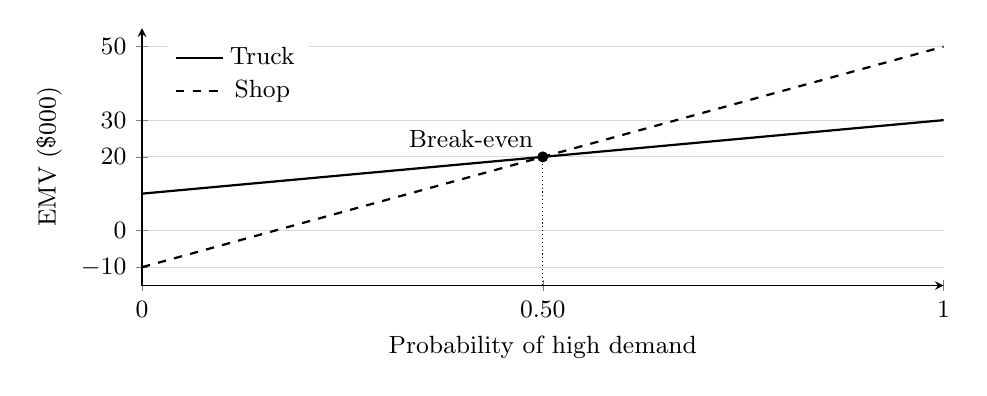
\begin{tikzpicture}
  \begin{axis}[
    width=0.97\linewidth,height=4.85cm,
    xmin=0,xmax=1,ymin=-15,ymax=55,
    axis lines=left,
    xlabel={Probability of high demand},ylabel={EMV (\$000)},
    xtick={0,0.5,1},xticklabels={\(0\),\(0.50\),\(1\)},
    ytick={-10,0,20,30,50},
    ymajorgrids,grid style={black!15},
    label style={font=\small},tick label style={font=\small},
    legend style={at={(0.03,0.97)},anchor=north west,font=\small,draw=none}
  ]
    \addplot[black,thick] coordinates {(0,10) (1,30)};
    \addlegendentry{Truck}
    \addplot[black,thick,dashed] coordinates {(0,-10) (1,50)};
    \addlegendentry{Shop}
    \draw[densely dotted] (axis cs:0.5,-15) -- (axis cs:0.5,20);
    \fill (axis cs:0.5,20) circle[radius=2pt];
    \node[font=\small,anchor=south east] at (axis cs:0.5,20) {Break-even};
  \end{axis}
\end{tikzpicture}
\end{minipage}\par

At break-even, \(10+20p=-10+60p\), so \(p=0.50\) and both EMVs are 20.
Truck is preferred below \(0.50\) and Shop is preferred above \(0.50\).

\begin{criteria}
  \criterion{C6}{Calculates Expected Monetary Value using stated or estimated probabilities and applies the Bayes decision criterion to select the alternative with the highest expected payoff.}
  \criterion{C7}{Uses subjective probabilities and sensitivity analysis to examine how changes in probability assumptions affect the preferred decision.}
\end{criteria}

\clearpage
\section{Compare criteria and build filtering trees}
Explain why the four rules can recommend different alternatives. Then draw a filtering tree, applying each rule in order using the given statistics for the alternatives still in contention.

\subsection*{C8 \textemdash{} Repair Workshop Plans (Q1, thousands of USD)}
{\small
\begin{tabularx}{\linewidth}{@{}lllL@{}}
\toprule
Rule & Recommendation & Statistic & Priority and limitation\\
\midrule
Maximax & Large & Row maximum 120 & Pursues the highest payoff. Ignores downside.\\
Maximin & Basic & Row minimum 35 & Picks the best worst-case payoff. Ignores upside.\\
Minimax Regret & Flexible & Maximum regret 45 & Minimises the worst missed profit. Depends on which alternatives set the benchmarks.\\
EMV/Bayes & Partner & EMV 63 & Maximises expected profit. Depends on reliable probabilities.\\
\bottomrule
\end{tabularx}\par}
Only EMV/Bayes weights payoffs by state probabilities. The other rules compare payoff extremes or regret directly.

Eligibility rules and payoff changes can change the choice. In \textbf{Community Market Stall (Q2)}, only Compact and Standard meet the payoff floor. Use their updated payoffs to recalculate each state's best payoff before finding regret.

\subsection*{C9 \textemdash{} Book Fair Stock (Q3, hundreds of USD)}
\begin{center}
\begin{tikzpicture}[node distance=23mm]
  \node[outline box] (start) {Start\\\(D_1\)--\(D_6\)};
  \node[outline box,right=of start] (keep1) {Keep \(D_1,D_2,D_3\)\\All tied at 65};
  \node[outline box,right=of keep1] (keep2) {Keep \(D_1\) (100)\\and \(D_2\) (90)};
  \node[outline box,right=of keep2,fill=black!8] (select) {\textbf{Select \(D_2\)}\\Minimum 10};
  \draw[outline arrow] (start) -- coordinate[midway] (rule1) (keep1);
  \draw[outline arrow] (keep1) -- coordinate[midway] (rule2) (keep2);
  \draw[outline arrow] (keep2) -- coordinate[midway] (rule3) (select);
  \node[above=5mm of rule1,font=\small\bfseries] {1. EMV/Bayes};
  \node[above=5mm of rule2,font=\small\bfseries] {2. Maximax};
  \node[above=5mm of rule3,font=\small\bfseries] {3. Maximin};
  \node[outline box,below=7mm of rule1] (drop1) {Drop \(D_4,D_5,D_6\)};
  \node[outline box,below=7mm of rule2] (drop2) {Drop \(D_3\) (80)};
  \node[outline box,below=7mm of rule3] (drop3) {Drop \(D_1\)\\Minimum 0};
  \draw[outline drop] (rule1) -- (drop1);
  \draw[outline drop] (rule2) -- (drop2);
  \draw[outline drop] (rule3) -- (drop3);
\end{tikzpicture}
\end{center}

\begin{criteria}
  \criterion{C8}{Compares the Maximax, Maximin, Minimax Regret, and EMV/Bayes decision criteria by contrasting their information requirements, risk orientations, recommended alternatives, and limitations.}
  \criterion{C9}{Constructs and interprets decision trees for staged filtering rules, applying decision criteria in the specified order to identify the final alternative.}
\end{criteria}

\section{Evaluate and justify the decision}
For the economic or financial scenario, select and justify the most appropriate criterion using the available information, risk attitude, and decision context.

\subsection*{C10 \textemdash{} A small café turns evidence into a defensible investment decision}
\begin{center}
\begin{tikzpicture}[node distance=6mm]
  \node[outline box] (survey) {\textbf{Market survey}\\Demand data};
  \node[outline box,right=of survey] (evidence)
    {\textbf{Financial evidence}\\Revenue, fixed costs,\\variable costs\\and probabilities};
  \node[outline box,right=of evidence] (compare)
    {\textbf{Compare criteria}\\and risk limits};
  \node[outline box,right=of compare,fill=black!8] (launch) {\textbf{Justify launch}};
  \draw[outline arrow] (survey) -- (evidence);
  \draw[outline arrow] (evidence) -- (compare);
  \draw[outline arrow] (compare) -- (launch);
\end{tikzpicture}\par
\smallskip
\small Real constraints include loan repayments, jobs, and cash-flow survival.
\end{center}

\begin{criteria}
  \criterion{C10}{Evaluates economic and financial decision-making scenarios by selecting and justifying the most appropriate decision criterion according to the information available, risk attitude, and decision context.}
\end{criteria}

\end{document}
